%% LyX 2.2.1 created this file.  For more info, see http://www.lyx.org/.
%% Do not edit unless you really know what you are doing.
\documentclass[a4paper,12pt,titlepage,microtype,hyperref,english]{article}
\usepackage[margin=1.3in]{geometry}
\usepackage[T1]{fontenc}
\usepackage[latin9]{luainputenc}
\usepackage{graphicx}
\usepackage{babel}
\usepackage{amsmath}
\usepackage{gensymb}
\usepackage[colorlinks,bookmarks=false,linkcolor=blue,urlcolor=blue]{hyperref}

\begin{document}


\title{GENOMIC PROJECT}
\author{Genom-1 Group}  %Don't know if it's nice ?


\maketitle
\tableofcontents

\baselineskip=16pt
\parindent=15pt
\parskip=5pt

\section{Introduction}

We were given the objective to build a program with actual applications
in current genomic problems. Several resource files can be given by the user,
such as a genomic sequence, a Position Weight Matrix (PWM) or Position-Specific Scoring Matrix (PSSM), affinity
scores along a specific sequence\ldots The idea is to offer different
outputs that can help the user to solve his/her problem. The output can
be a list of binding sites present in a chromosome, an affinity score for a given binding site, a PWM (or
a PSSM), or a graphic representation of the consensus sequence determined by the PMW (a logo showing the
different nucleotides A, T, C and G, their sizes representing their respective probability). 

\begin{figure}[!h]
\caption{Example of a PWM matrix.}
\centering{}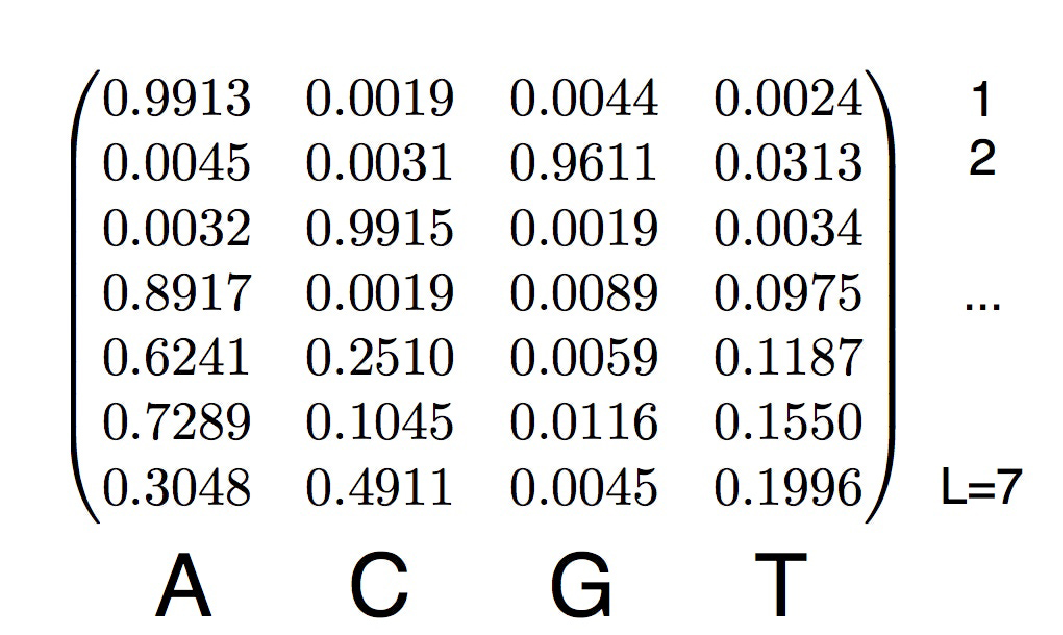
\includegraphics[scale=0.5]{ImagesREADME/PWM.pdf}
\end{figure}

\begin{figure}[!h]
\noindent \caption{Logo of a consensus sequence.}
\noindent \centering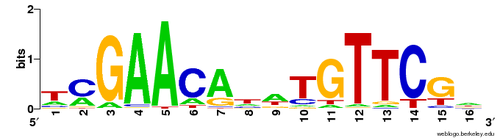
\includegraphics[scale=0.7]{ImagesREADME/Logo}
\end{figure}


\section{Download the program}

To download the program, go to : \url{https://github.com/EPFL-SV-cpp-projects/genom-1}.
Open a terminal and go to the directory where you want the program, then type "git clone~\textbf{https://github.com/EPFL-SV-cpp-projects/genom-1''.
}The genom-1 folder and all of its content will be copied into your directory,
you can then compile and execute the program.

\section{Compilation and execution}

To compile and execute the program, a fews steps are required. Make
sure you are in the genom-1 folder and then :

\textbf{rm \textendash rf build }and\textbf{ mkdir build} to make
sure an empty build folder is crated

\textbf{cmake../ }

\textbf{make}

And then you have several options

If you want to see the documentation with the doxyfile, describing
more precisely the different classes and fonctions involved in the
program you will then have to write \textbf{make doc}

If you want to execute the program, then do \textbf{../src/Main}

If you want to run the tests of the program, then do \textbf{make
test}

\section{The functionalities of the program }

When you execute the program, a menu will appear, proposing you a
list of outputs designed by their numbers. You can choose the task
the program must do by hitting '1', '2' or '3' or '4'. Then you will
be asked to provide the inputs (if the program needs a file you can
write its name like \textquotedbl{}$example.fasta$\textquotedbl{}).
Here are the mains functionalities of the program :

1.- Being able to read a DNA sequence and a PWM (or/and it's logarithmic
version) and give as output the list of site along the genome where
the protein is gonna attach.

2.- Being able to read a DNA sequence, a list of sites and their respective
binding score (the product of the probabilities of each nucleotide
along the sequence) and output a PWM (or/and it's logarithmic version).

3.- Based on the matrix or based on the binding scores and list of
sites, being able produce a sequence logo.


\end{document}
